\documentclass{article}
\usepackage{rotating}

\usepackage{tikz}
\usepackage{graphicx}
\usepackage{fontspec}
\usepackage{tocloft}
\usepackage{titletoc}
\usepackage{lipsum}  

\setmainfont{LEMONMILK-Bold.otf}[Path=Assets/Fonts/]

\begin{document}
%%%%%%%%%%    COVER    %%%%%%%%%%
\begin{titlepage}
\begin{tikzpicture}[remember picture,overlay]
    \fill[color=black] (current page.north west) rectangle ++(5cm,-\paperheight);
    \node[anchor=south west, text=white] at (current page.south west) {\hspace{1.5cm}\begin{turn}{90}
    \resizebox{!}{35.5pt}{\hspace{1.17cm}Intellinterpreter}\end{turn}};
\end{tikzpicture}

\begin{flushright}

\vspace{3cm}

\Huge Fundamentos Computacionales: Un Análisis Detallado del Intellinterpreter para el Lenguaje Hulk

\vspace{1.5cm}

\Large Raciel Pupo Santos

\vspace{5cm}

\normalsize jul 17th, 2023

\end{flushright}

\end{titlepage}
\newpage
%%%%%%%%%%%%%%%%%%%%%%%%%%%%%%%%%
%%%%%%%%%%    LIST OF CONTENTS    %%%%%%%%%%
\tableofcontents
\newpage
%%%%%%%%%%%%%%%%%%%%%%%%%%%%%%%%%
%%%%%%%%%%    CONTENT    %%%%%%%%%%
\setmainfont{LEMONMILK-Bold.otf}[Path=Assets/Fonts/]
\section{Introducción}
    \setmainfont{LEMONMILK-Regular.otf}[Path=Assets/Fonts/]
    ¡Bienvenidos a la presentación del Intérprete Hulk! Este sistema de procesamiento de lenguajes está diseñado para interpretar programas escritos en el lenguaje de programación Hulk. A través de una combinación de principios informáticos y fundamentos matemáticos, el Intérprete Hulk se alza como una herramienta robusta y versátil para analizar y ejecutar código en este emocionante lenguaje.
\newpage

\setmainfont{LEMONMILK-Bold.otf}[Path=Assets/Fonts/]
\section{Lexer - Tokenizando el Código Fuente}
    \setmainfont{LEMONMILK-Regular.otf}[Path=Assets/Fonts/]
    En el corazón del Intérprete Hulk se encuentra el Lexer, el analizador léxico, que realiza una tarea crucial: tokenizar el código fuente. Mediante el uso de un autómata finito, el Lexer identifica palabras clave, identificadores, literales y símbolos, entre otros elementos. Esta tokenización crea una representación estructurada y significativa del código fuente, permitiendo fases posteriores de interpretación.
    \begin{figure}[ht]
        \centering
        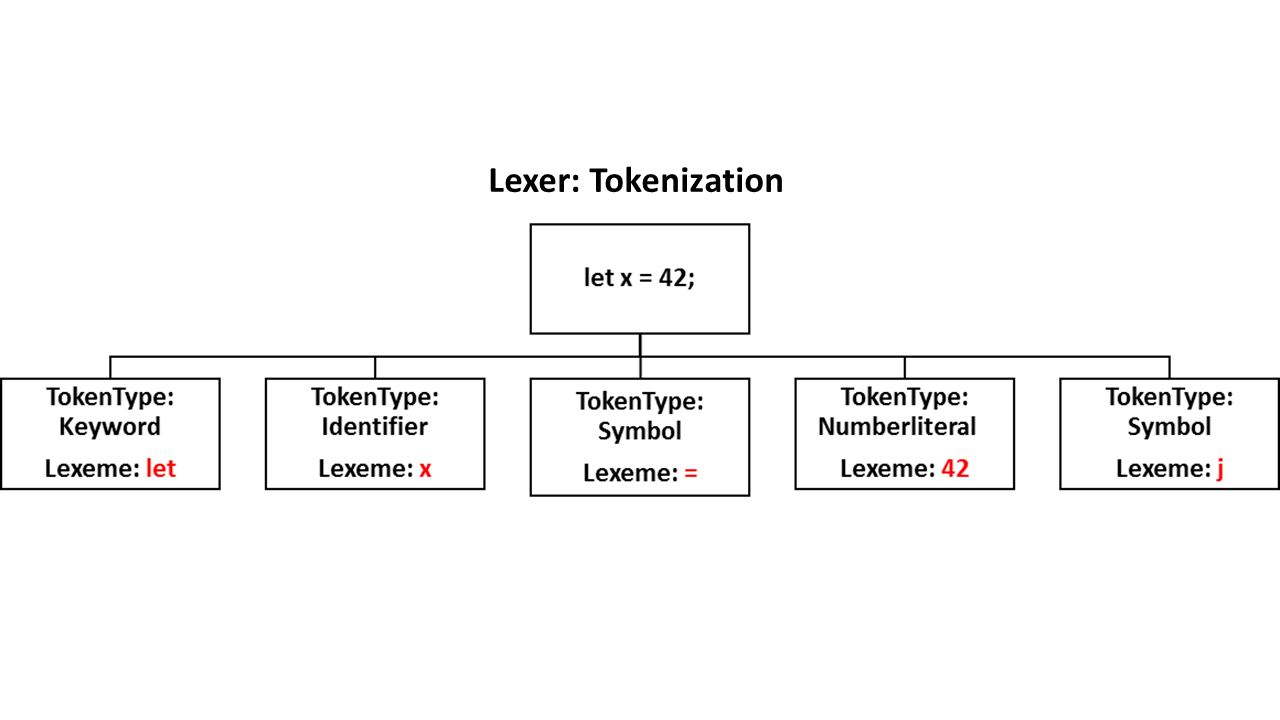
\includegraphics[width=0.5\linewidth]{Assets/Tokenization.png} % Asegúrate de tener el archivo de la imagen en el mismo directorio o ajusta la ruta aquí.
        \caption{Proceso de Tokenización (Analizador Léxico)}
        \label{fig:tokenizacion}
    \end{figure}
\newpage

\setmainfont{LEMONMILK-Bold.otf}[Path=Assets/Fonts/]
\section{Parser - Construyendo el Árbol de Sintaxis Abstracta (AST)}
    \setmainfont{LEMONMILK-Regular.otf}[Path=Assets/Fonts/]
    El Parser, componente clave del Intérprete Hulk, es responsable de construir el Árbol de Sintaxis Abstracta (AST) a partir de la secuencia de tokens generada por el Lexer. El AST es una representación jerárquica de la sintaxis y semántica del programa, que guía al intérprete en la ejecución precisa del código Hulk. Mediante el enfoque de análisis descendente recursivo, el Parser examina meticulosamente cada token, creando nodos en el AST que reflejan con precisión la precedencia y asociatividad de los operadores.
    \begin{figure}[ht]
        \centering
        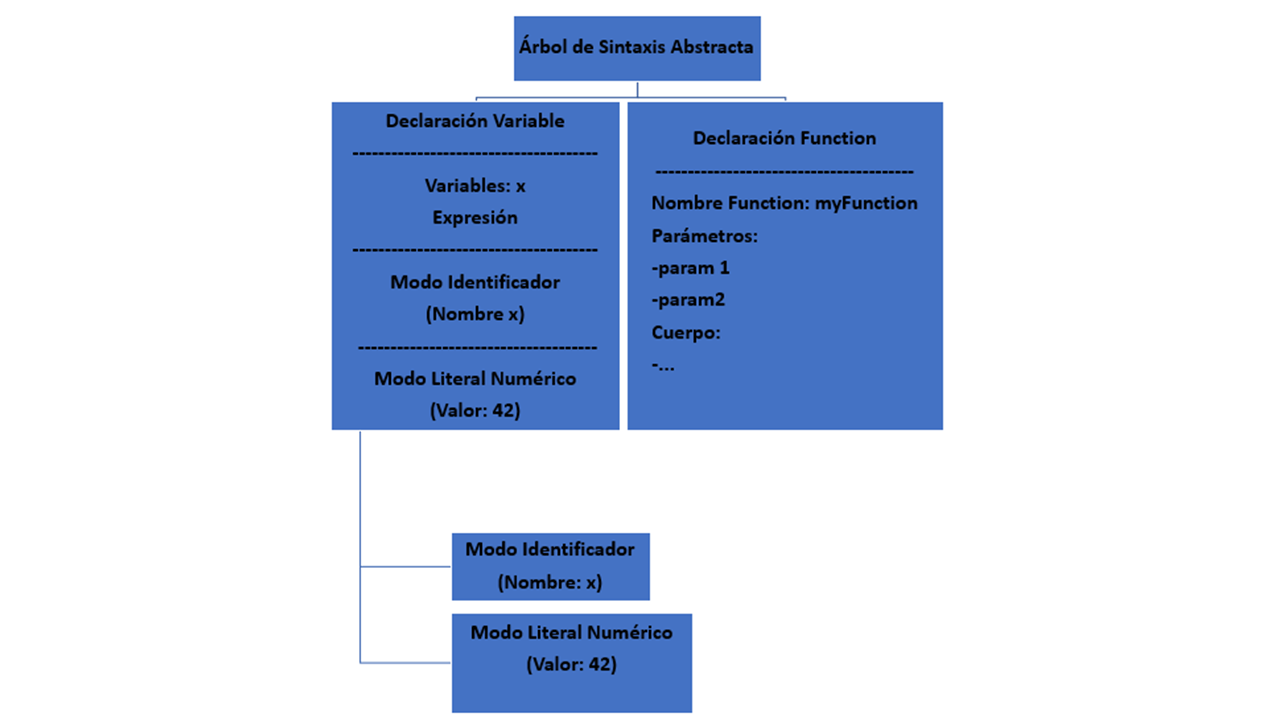
\includegraphics[width=0.5\linewidth]{Assets/ArboldeSintaxisAbstracta.png} % Asegúrate de tener el archivo de la imagen en el mismo directorio o ajusta la ruta aquí.
        \caption{Construcción del AST}
        \label{fig:AST}
    \end{figure}
\newpage

\setmainfont{LEMONMILK-Bold.otf}[Path=Assets/Fonts/]
\section{Analizador Semántico - Garantizando la Semántica del Programa}
    \setmainfont{LEMONMILK-Regular.otf}[Path=Assets/Fonts/]
    El Analizador Semántico se presenta como el guardián, protegiendo contra inconsistencias semánticas en el programa Hulk. Operando sobre el AST creado por el Parser, el analizador escruta las referencias de variables, las declaraciones de funciones y la compatibilidad de tipos de expresiones. Las tablas de variables y funciones desempeñan un papel vital, permitiendo al analizador semántico rastrear meticulosamente las variables y funciones definidas en el programa.
    \begin{figure}[ht]
        \centering
        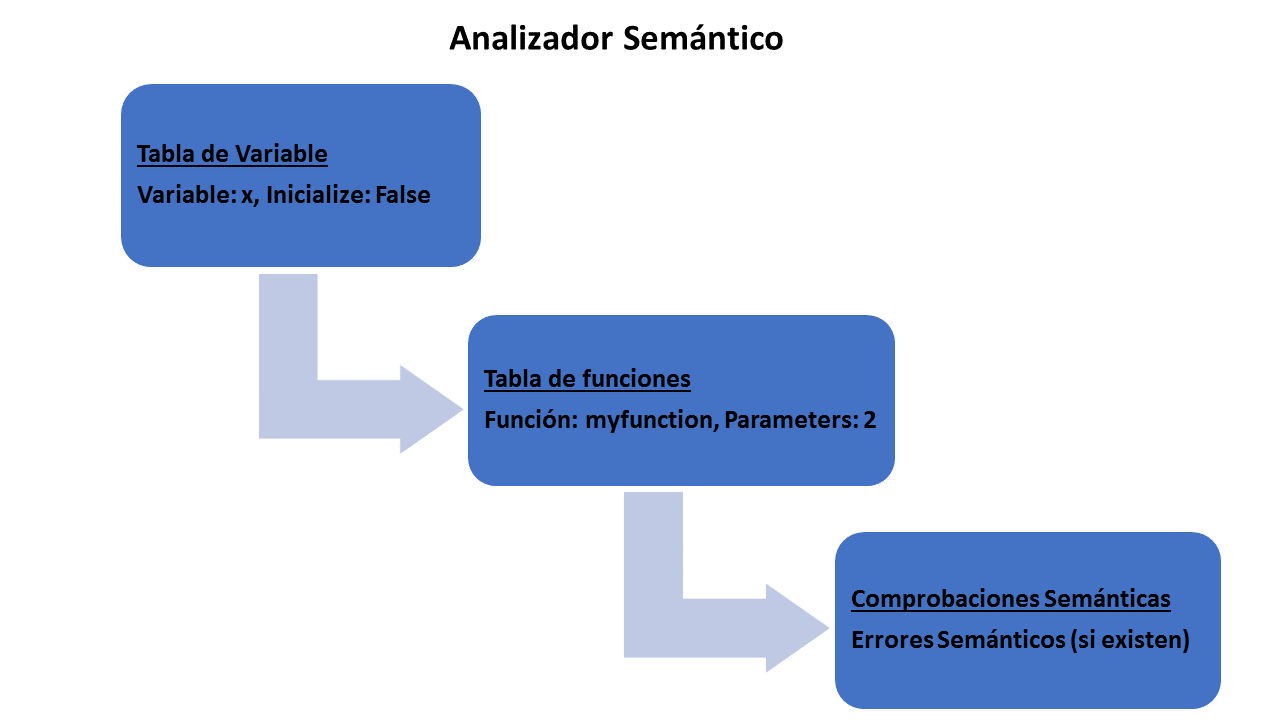
\includegraphics[width=0.5\linewidth]{Assets/AnalizadorSemantico.png} % Asegúrate de tener el archivo de la imagen en el mismo directorio o ajusta la ruta aquí.
        \caption{Proceso del Analizador Semantico}
        \label{fig:Asemantico}
    \end{figure}
    % \subsection{Feature 1}
    %     \lipsum[2-4]
    % \subsection{Feature 2}
    %     \lipsum[2-4]
    % \subsection{Feature 3}
    %     \lipsum[2-4]
\newpage

\setmainfont{LEMONMILK-Bold.otf}[Path=Assets/Fonts/]
\section{ Comprobaciones Semánticas Estáticas - Eliminando Errores}
    \setmainfont{LEMONMILK-Regular.otf}[Path=Assets/Fonts/]
    Tras la análisis semántico, las comprobaciones semánticas estáticas entran en juego. Su objetivo es identificar errores semánticos en el código antes de la ejecución. Si se encuentran errores, el intérprete puede notificar al programador y evitar comportamientos inesperados durante la interpretación.
    % \subsection{Item 1}
    %     \lipsum[2-4]
    % \subsection{Item 2}
    %     \lipsum[2-4]
    % \subsection{Item 3}
    %     \lipsum[2-4]
\newpage

\setmainfont{LEMONMILK-Bold.otf}[Path=Assets/Fonts/]
\section{Conclusiones - La Potencia del Intérprete Hulk}
    \setmainfont{LEMONMILK-Regular.otf}[Path=Assets/Fonts/]
    El Intérprete Hulk se erige como una herramienta poderosa y bien estructurada para el procesamiento de lenguajes. Su adhesión a principios informáticos y ecuaciones matemáticas que rigen la precedencia de operadores durante el análisis demuestran la robustez y eficiencia del Intérprete Hulk. Su diseño modular y uso de Árboles de Sintaxis Abstracta exponen la elegancia de los algoritmos de análisis. Con esta base, el futuro ofrece un vasto potencial para nuevos avances en el lenguaje Hulk y el intérprete.
\newpage

%%%%%%%%%%%%%%%%%%%%%%%%%%%%%%%%%
\end{document}

\begin{comment}

\end{comment}